


% Header, overrides base

    % Make sure that the sphinx doc style knows who it inherits from.
    \def\sphinxdocclass{article}

    % Declare the document class
  \documentclass[twocolumn,10pt,russian]{/usr/lib/python3.3/site-packages/sphinx/texinputs/sphinxhowto}
      \usepackage{wrapfig}
      \usepackage{mathrsfs}
      \usepackage{subcaption}
      \usepackage{placeins}
    % Imports
    \usepackage[utf8]{inputenc}
    \DeclareUnicodeCharacter{00A0}{\\nobreakspace}
    \usepackage[T1]{fontenc}
    \usepackage{babel}
    \usepackage{times}
    \usepackage{import}
    \usepackage[Bjarne]{/usr/lib/python3.3/site-packages/sphinx/texinputs/fncychap}
    \usepackage{longtable}
    \usepackage{/usr/lib/python3.3/site-packages/sphinx/texinputs/sphinx}
    \usepackage{multirow}

    \usepackage{amsmath}
    \usepackage{amssymb}
    \usepackage{ucs}
    \usepackage{enumerate}

    % Used to make the Input/Output rules follow around the contents.
    \usepackage{needspace}

    % Pygments requirements
    \usepackage{fancyvrb}
    \usepackage{color}
    % ansi colors additions
    \definecolor{darkgreen}{rgb}{.12,.54,.11}
    \definecolor{lightgray}{gray}{.95}
    \definecolor{brown}{rgb}{0.54,0.27,0.07}
    \definecolor{purple}{rgb}{0.5,0.0,0.5}
    \definecolor{darkgray}{gray}{0.25}
    \definecolor{lightred}{rgb}{1.0,0.39,0.28}
    \definecolor{lightgreen}{rgb}{0.48,0.99,0.0}
    \definecolor{lightblue}{rgb}{0.53,0.81,0.92}
    \definecolor{lightpurple}{rgb}{0.87,0.63,0.87}
    \definecolor{lightcyan}{rgb}{0.5,1.0,0.83}

    % Needed to box output/input
    \usepackage{tikz}
        \usetikzlibrary{calc,arrows,shadows}
    \usepackage[framemethod=tikz]{mdframed}

    \usepackage{alltt}

    % Used to load and display graphics
    \usepackage{graphicx}
    \graphicspath{ {figs/} }
    \usepackage[Export]{adjustbox} % To resize

    % used so that images for notebooks which have spaces in the name can still be included
    \usepackage{grffile}


    % For formatting output while also word wrapping.
    \usepackage{listings}
    \lstset{breaklines=true}
    \lstset{basicstyle=\small\ttfamily}
    \def\smaller{\fontsize{9.5pt}{9.5pt}\selectfont}

    %Pygments definitions
    
\makeatletter
\def\PY@reset{\let\PY@it=\relax \let\PY@bf=\relax%
    \let\PY@ul=\relax \let\PY@tc=\relax%
    \let\PY@bc=\relax \let\PY@ff=\relax}
\def\PY@tok#1{\csname PY@tok@#1\endcsname}
\def\PY@toks#1+{\ifx\relax#1\empty\else%
    \PY@tok{#1}\expandafter\PY@toks\fi}
\def\PY@do#1{\PY@bc{\PY@tc{\PY@ul{%
    \PY@it{\PY@bf{\PY@ff{#1}}}}}}}
\def\PY#1#2{\PY@reset\PY@toks#1+\relax+\PY@do{#2}}

\expandafter\def\csname PY@tok@kp\endcsname{\def\PY@tc##1{\textcolor[rgb]{0.00,0.50,0.00}{##1}}}
\expandafter\def\csname PY@tok@ni\endcsname{\let\PY@bf=\textbf\def\PY@tc##1{\textcolor[rgb]{0.60,0.60,0.60}{##1}}}
\expandafter\def\csname PY@tok@cm\endcsname{\let\PY@it=\textit\def\PY@tc##1{\textcolor[rgb]{0.25,0.50,0.50}{##1}}}
\expandafter\def\csname PY@tok@kt\endcsname{\def\PY@tc##1{\textcolor[rgb]{0.69,0.00,0.25}{##1}}}
\expandafter\def\csname PY@tok@gu\endcsname{\let\PY@bf=\textbf\def\PY@tc##1{\textcolor[rgb]{0.50,0.00,0.50}{##1}}}
\expandafter\def\csname PY@tok@vc\endcsname{\def\PY@tc##1{\textcolor[rgb]{0.10,0.09,0.49}{##1}}}
\expandafter\def\csname PY@tok@gp\endcsname{\let\PY@bf=\textbf\def\PY@tc##1{\textcolor[rgb]{0.00,0.00,0.50}{##1}}}
\expandafter\def\csname PY@tok@gs\endcsname{\let\PY@bf=\textbf}
\expandafter\def\csname PY@tok@gr\endcsname{\def\PY@tc##1{\textcolor[rgb]{1.00,0.00,0.00}{##1}}}
\expandafter\def\csname PY@tok@kc\endcsname{\let\PY@bf=\textbf\def\PY@tc##1{\textcolor[rgb]{0.00,0.50,0.00}{##1}}}
\expandafter\def\csname PY@tok@vi\endcsname{\def\PY@tc##1{\textcolor[rgb]{0.10,0.09,0.49}{##1}}}
\expandafter\def\csname PY@tok@gi\endcsname{\def\PY@tc##1{\textcolor[rgb]{0.00,0.63,0.00}{##1}}}
\expandafter\def\csname PY@tok@nl\endcsname{\def\PY@tc##1{\textcolor[rgb]{0.63,0.63,0.00}{##1}}}
\expandafter\def\csname PY@tok@cp\endcsname{\def\PY@tc##1{\textcolor[rgb]{0.74,0.48,0.00}{##1}}}
\expandafter\def\csname PY@tok@ge\endcsname{\let\PY@it=\textit}
\expandafter\def\csname PY@tok@gd\endcsname{\def\PY@tc##1{\textcolor[rgb]{0.63,0.00,0.00}{##1}}}
\expandafter\def\csname PY@tok@cs\endcsname{\let\PY@it=\textit\def\PY@tc##1{\textcolor[rgb]{0.25,0.50,0.50}{##1}}}
\expandafter\def\csname PY@tok@il\endcsname{\def\PY@tc##1{\textcolor[rgb]{0.40,0.40,0.40}{##1}}}
\expandafter\def\csname PY@tok@kn\endcsname{\let\PY@bf=\textbf\def\PY@tc##1{\textcolor[rgb]{0.00,0.50,0.00}{##1}}}
\expandafter\def\csname PY@tok@sx\endcsname{\def\PY@tc##1{\textcolor[rgb]{0.00,0.50,0.00}{##1}}}
\expandafter\def\csname PY@tok@mi\endcsname{\def\PY@tc##1{\textcolor[rgb]{0.40,0.40,0.40}{##1}}}
\expandafter\def\csname PY@tok@mh\endcsname{\def\PY@tc##1{\textcolor[rgb]{0.40,0.40,0.40}{##1}}}
\expandafter\def\csname PY@tok@mo\endcsname{\def\PY@tc##1{\textcolor[rgb]{0.40,0.40,0.40}{##1}}}
\expandafter\def\csname PY@tok@ss\endcsname{\def\PY@tc##1{\textcolor[rgb]{0.10,0.09,0.49}{##1}}}
\expandafter\def\csname PY@tok@sr\endcsname{\def\PY@tc##1{\textcolor[rgb]{0.73,0.40,0.53}{##1}}}
\expandafter\def\csname PY@tok@mf\endcsname{\def\PY@tc##1{\textcolor[rgb]{0.40,0.40,0.40}{##1}}}
\expandafter\def\csname PY@tok@si\endcsname{\let\PY@bf=\textbf\def\PY@tc##1{\textcolor[rgb]{0.73,0.40,0.53}{##1}}}
\expandafter\def\csname PY@tok@sh\endcsname{\def\PY@tc##1{\textcolor[rgb]{0.73,0.13,0.13}{##1}}}
\expandafter\def\csname PY@tok@ow\endcsname{\let\PY@bf=\textbf\def\PY@tc##1{\textcolor[rgb]{0.67,0.13,1.00}{##1}}}
\expandafter\def\csname PY@tok@gt\endcsname{\def\PY@tc##1{\textcolor[rgb]{0.00,0.27,0.87}{##1}}}
\expandafter\def\csname PY@tok@sc\endcsname{\def\PY@tc##1{\textcolor[rgb]{0.73,0.13,0.13}{##1}}}
\expandafter\def\csname PY@tok@sb\endcsname{\def\PY@tc##1{\textcolor[rgb]{0.73,0.13,0.13}{##1}}}
\expandafter\def\csname PY@tok@se\endcsname{\let\PY@bf=\textbf\def\PY@tc##1{\textcolor[rgb]{0.73,0.40,0.13}{##1}}}
\expandafter\def\csname PY@tok@sd\endcsname{\let\PY@it=\textit\def\PY@tc##1{\textcolor[rgb]{0.73,0.13,0.13}{##1}}}
\expandafter\def\csname PY@tok@m\endcsname{\def\PY@tc##1{\textcolor[rgb]{0.40,0.40,0.40}{##1}}}
\expandafter\def\csname PY@tok@nd\endcsname{\def\PY@tc##1{\textcolor[rgb]{0.67,0.13,1.00}{##1}}}
\expandafter\def\csname PY@tok@kr\endcsname{\let\PY@bf=\textbf\def\PY@tc##1{\textcolor[rgb]{0.00,0.50,0.00}{##1}}}
\expandafter\def\csname PY@tok@vg\endcsname{\def\PY@tc##1{\textcolor[rgb]{0.10,0.09,0.49}{##1}}}
\expandafter\def\csname PY@tok@bp\endcsname{\def\PY@tc##1{\textcolor[rgb]{0.00,0.50,0.00}{##1}}}
\expandafter\def\csname PY@tok@c1\endcsname{\let\PY@it=\textit\def\PY@tc##1{\textcolor[rgb]{0.25,0.50,0.50}{##1}}}
\expandafter\def\csname PY@tok@nb\endcsname{\def\PY@tc##1{\textcolor[rgb]{0.00,0.50,0.00}{##1}}}
\expandafter\def\csname PY@tok@nc\endcsname{\let\PY@bf=\textbf\def\PY@tc##1{\textcolor[rgb]{0.00,0.00,1.00}{##1}}}
\expandafter\def\csname PY@tok@o\endcsname{\def\PY@tc##1{\textcolor[rgb]{0.40,0.40,0.40}{##1}}}
\expandafter\def\csname PY@tok@na\endcsname{\def\PY@tc##1{\textcolor[rgb]{0.49,0.56,0.16}{##1}}}
\expandafter\def\csname PY@tok@nf\endcsname{\def\PY@tc##1{\textcolor[rgb]{0.00,0.00,1.00}{##1}}}
\expandafter\def\csname PY@tok@err\endcsname{\def\PY@bc##1{\setlength{\fboxsep}{0pt}\fcolorbox[rgb]{1.00,0.00,0.00}{1,1,1}{\strut ##1}}}
\expandafter\def\csname PY@tok@k\endcsname{\let\PY@bf=\textbf\def\PY@tc##1{\textcolor[rgb]{0.00,0.50,0.00}{##1}}}
\expandafter\def\csname PY@tok@ne\endcsname{\let\PY@bf=\textbf\def\PY@tc##1{\textcolor[rgb]{0.82,0.25,0.23}{##1}}}
\expandafter\def\csname PY@tok@s1\endcsname{\def\PY@tc##1{\textcolor[rgb]{0.73,0.13,0.13}{##1}}}
\expandafter\def\csname PY@tok@go\endcsname{\def\PY@tc##1{\textcolor[rgb]{0.53,0.53,0.53}{##1}}}
\expandafter\def\csname PY@tok@s2\endcsname{\def\PY@tc##1{\textcolor[rgb]{0.73,0.13,0.13}{##1}}}
\expandafter\def\csname PY@tok@nn\endcsname{\let\PY@bf=\textbf\def\PY@tc##1{\textcolor[rgb]{0.00,0.00,1.00}{##1}}}
\expandafter\def\csname PY@tok@no\endcsname{\def\PY@tc##1{\textcolor[rgb]{0.53,0.00,0.00}{##1}}}
\expandafter\def\csname PY@tok@c\endcsname{\let\PY@it=\textit\def\PY@tc##1{\textcolor[rgb]{0.25,0.50,0.50}{##1}}}
\expandafter\def\csname PY@tok@nv\endcsname{\def\PY@tc##1{\textcolor[rgb]{0.10,0.09,0.49}{##1}}}
\expandafter\def\csname PY@tok@nt\endcsname{\let\PY@bf=\textbf\def\PY@tc##1{\textcolor[rgb]{0.00,0.50,0.00}{##1}}}
\expandafter\def\csname PY@tok@w\endcsname{\def\PY@tc##1{\textcolor[rgb]{0.73,0.73,0.73}{##1}}}
\expandafter\def\csname PY@tok@kd\endcsname{\let\PY@bf=\textbf\def\PY@tc##1{\textcolor[rgb]{0.00,0.50,0.00}{##1}}}
\expandafter\def\csname PY@tok@s\endcsname{\def\PY@tc##1{\textcolor[rgb]{0.73,0.13,0.13}{##1}}}
\expandafter\def\csname PY@tok@gh\endcsname{\let\PY@bf=\textbf\def\PY@tc##1{\textcolor[rgb]{0.00,0.00,0.50}{##1}}}

\def\PYZbs{\char`\\}
\def\PYZus{\char`\_}
\def\PYZob{\char`\{}
\def\PYZcb{\char`\}}
\def\PYZca{\char`\^}
\def\PYZam{\char`\&}
\def\PYZlt{\char`\<}
\def\PYZgt{\char`\>}
\def\PYZsh{\char`\#}
\def\PYZpc{\char`\%}
\def\PYZdl{\char`\$}
\def\PYZhy{\char`\-}
\def\PYZsq{\char`\'}
\def\PYZdq{\char`\"}
\def\PYZti{\char`\~}
% for compatibility with earlier versions
\def\PYZat{@}
\def\PYZlb{[}
\def\PYZrb{]}
\makeatother


    %Set pygments styles if needed...
    
        \definecolor{nbframe-border}{rgb}{0.867,0.867,0.867}
        \definecolor{nbframe-bg}{rgb}{0.969,0.969,0.969}
        \definecolor{nbframe-in-prompt}{rgb}{0.0,0.0,0.502}
        \definecolor{nbframe-out-prompt}{rgb}{0.545,0.0,0.0}

        \newenvironment{ColorVerbatim}
        {\begin{mdframed}[%
            roundcorner=1.0pt, %
            backgroundcolor=nbframe-bg, %
            userdefinedwidth=1\linewidth, %
            leftmargin=0.1\linewidth, %
            innerleftmargin=0pt, %
            innerrightmargin=0pt, %
            linecolor=nbframe-border, %
            linewidth=1pt, %
            usetwoside=false, %
            everyline=true, %
            innerlinewidth=3pt, %
            innerlinecolor=nbframe-bg, %
            middlelinewidth=1pt, %
            middlelinecolor=nbframe-bg, %
            outerlinewidth=0.5pt, %
            outerlinecolor=nbframe-border, %
            needspace=0pt
        ]}
        {\end{mdframed}}
        
        \newenvironment{InvisibleVerbatim}
        {\begin{mdframed}[leftmargin=0.1\linewidth,innerleftmargin=3pt,innerrightmargin=3pt, userdefinedwidth=1\linewidth, linewidth=0pt, linecolor=white, usetwoside=false]}
        {\end{mdframed}}

        \renewenvironment{Verbatim}[1][\unskip]
        {\begin{alltt}\smaller}
        {\end{alltt}}
    

    % Help prevent overflowing lines due to urls and other hard-to-break 
    % entities.  This doesn't catch everything...
    \sloppy

    % Document level variables
    \title{SEM}
    \date{March 29, 2014}
    \release{}
    \author{Первая Группа}
    \renewcommand{\releasename}{}

    % TODO: Add option for the user to specify a logo for his/her export.
    \newcommand{\sphinxlogo}{}

    % Make the index page of the document.
    \makeindex

    % Import sphinx document type specifics.
     


% Body

    % Start of the document
    \begin{document}

        
    
\part*{Сканирующая электронная микроскопия}В работе были исследованы мембраны компании Whatman \textbf{Anodisc}
(анодированный алюминий). С заявленными производителем были сопоставлены
следующие параметры: толщина мембраны, диаметр пор, плотность пор.
Зафиксированы также отклонение пор от цилиндричности и отклонение
каналов от нормали к поверхности мембраны.
\section*{Введение}Мембраны анодированного алюминия могут использоваться в качестве матриц
для формирования металлических нанопроволок и нанопроводов. При таком
использовании являются важными особенности их геометрии, такие как
форма, размер пор, наклон каналов и количество дефектов. В данной работе
предметом исследования является мембрана компании Whatman
\textbf{Anodisc}, предназначенная для использования как фильтра, со
следующими заявленными усредненными параметрами:

\begin{itemize}
\itemsep1pt\parskip0pt\parsep0pt
\item
  толщина мембраны $22$ мкм
\item
  диаметр пор $0.1$ мкм
\item
  плотность пор $2\cdot 10^8$ см$^{-2}$
\end{itemize}Результатом нашей работы является сравнение реальных характеристик
мембраны с заявленными, а также определения качества полученных каналов
для установления пригодности их к использованию в качестве матриц для
выращивания металлических нанопроводов.

\section{Экспериментальная часть}
\subsection{Физический эксперимент}
Так как в процессе сканирующей электронной микроскопии образец
заряжается нам нужен проводящий слой на поверхности. В PVD-процессе был
напылен тонкий слой золота на поверхность мембраны. Затем образец был
помещен в микроскоп и была производена съёмка поверхностей. Фотографии можно видеть на Рис. 1

    

    \begin{figure}
    \centering
    \begin{subfigure}[t]{0.5\textwidth}
    \centering
    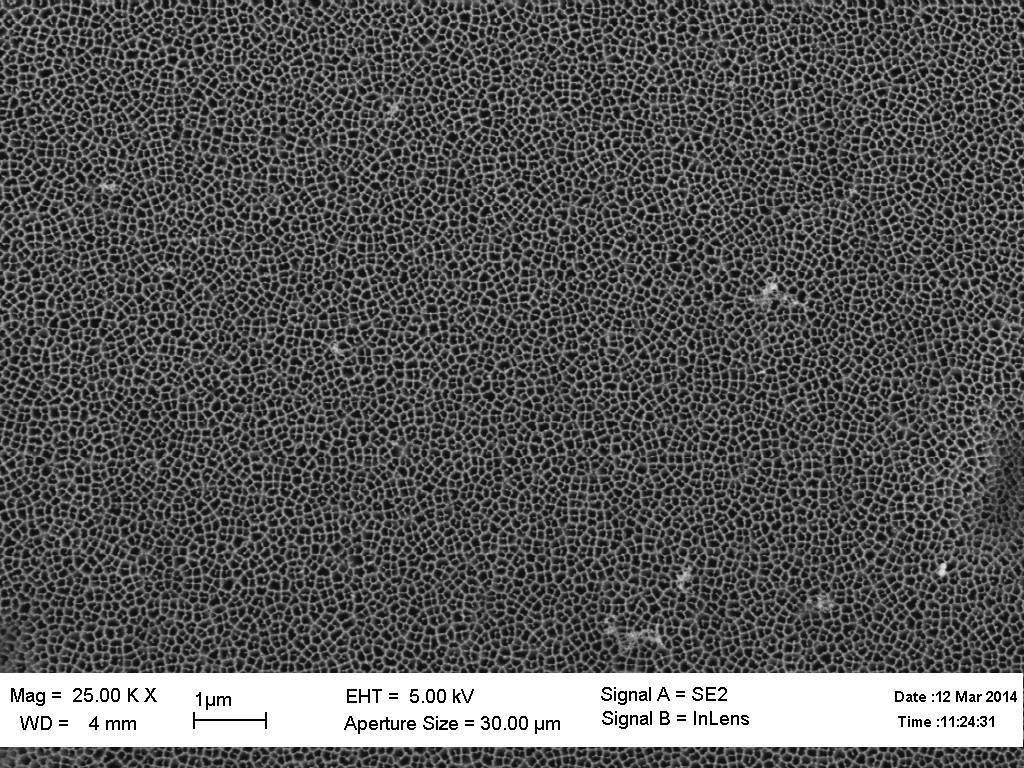
\includegraphics[max size={0.9\textwidth}{\textheight}]{PIL_Test_files/PIL_Test_10_0.jpeg}
    \caption{Вид мембраны сверху (верх соответствует верху на рис. (б))}
    \end{subfigure}
  
    
    \begin{subfigure}[t]{0.5\textwidth}
    \centering
    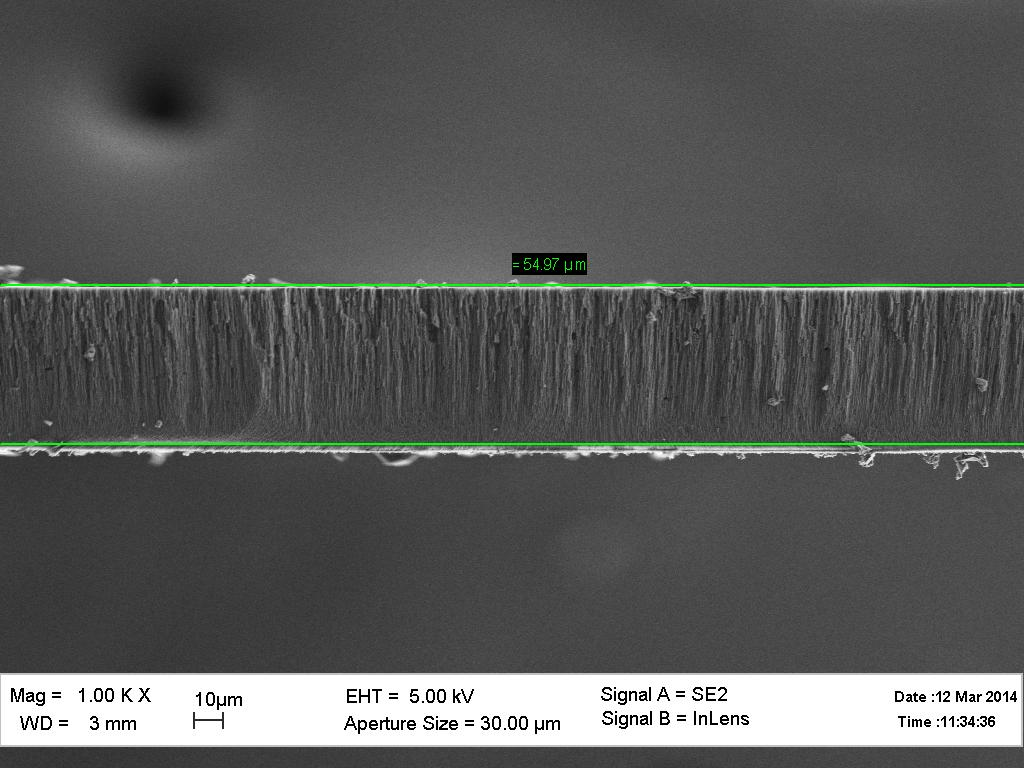
\includegraphics[max size={0.9\textwidth}{\textheight}]{PIL_Test_files/PIL_Test_11_0.jpeg}
    \caption{Вид скола при меньшем увеличении}
    \end{subfigure} 
    
    \begin{subfigure}{0.5\textwidth}
    \centering
    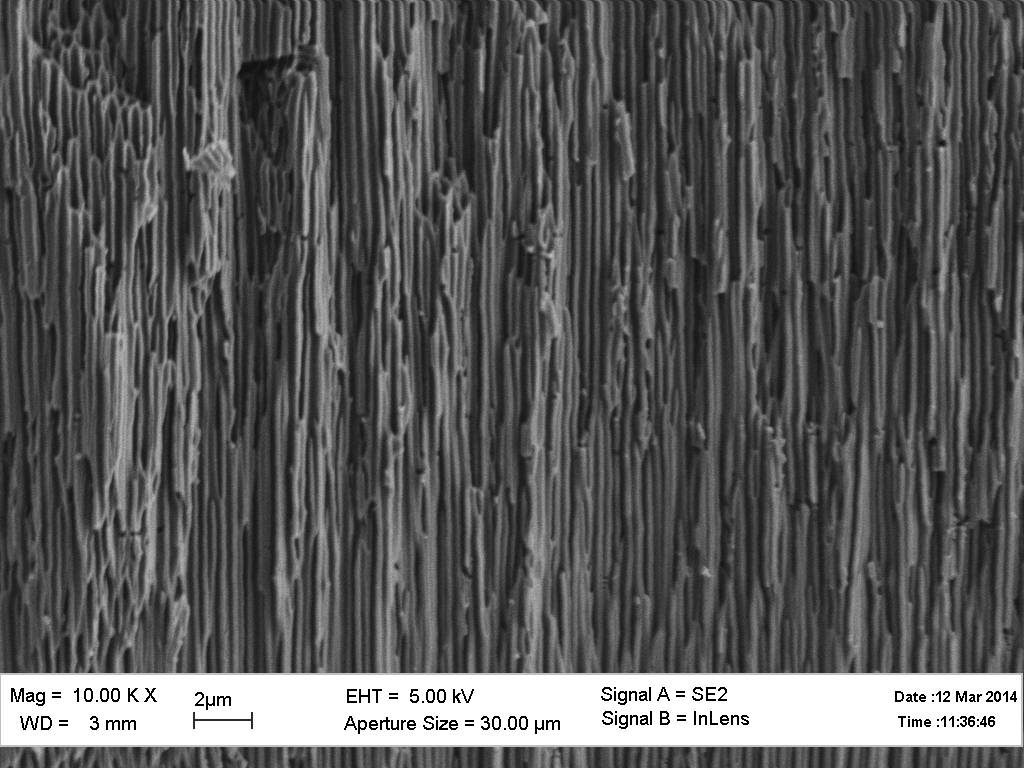
\includegraphics[max size={0.9\textwidth}{\textheight}]{PIL_Test_files/PIL_Test_12_0.jpeg}
    \caption{Вид части скола в толще мембраны при большем увеличении}
    \end{subfigure}
    
    \caption{Полученные снимки}
    \end{figure}
            
        \FloatBarrier
    
\subsection{Данные}Результатом эксперимента являются полученные изображения мембраны. Для
определения среднего диаметра пор и среднего угла их наклона в мембране
с помощью этих картин были написаны программы на языке Python. Ниже
приведены алгоритмы для каждой из задач. Для обеих задач необходима
предварительная обработка изображения. Сначала выделяется область
картинки, которая не содержит в себе данных о параметрах съемки и
масштабе, имеющиеся внизу изображения. Затем происходит перебор
пикселей. Те, значение которых больше некоторого порогового,
закрашиваются белым цетом, а остальные черным. Оптимальное пороговое
значение подбирается опытным путём. Таким образом происходит выделение
границы, и картинка становится контрастней (Рис. 2).
\subsubsection{Размеры пор}
После обработки у нас имеется набор черных пикселей, которые являются
внутренними по отношению к порам, и белые, которые принадлежат их
границе. Начинаем последовательный перебор пикселей. Если находим чёрный
пиксель, это значит, что мы нашли пору. Теперь находим все пиксели,
принадлежащие этой же поре, и добавляем их в множество, соотвествующее
этой поре. Это делается следующим образом: для первого черного пикселя
проверяется, все ли его ближайшие соседи являются черными. Если да, то
они добавляются в множество поры и закрашиваются серым, если нет, то
вновь продолжается поиск черных пикселей, т.е новых пор, причем уже
приписанные найденной поре пиксели уже точно выходят из повторного
рассмотрения, т.к. мы закрасили их серым) (Рис. 3). В итоге мы получаем множество
координат пикселей, принадлежащих каждой из найденных пор. Далее мы
находим размер пор как диаметр множества или как корень из площади поры.
Площадь поры вычисляется, как количество пикселей, принадлежащих ей,
умноженное на площадь одного пикселя (размер пикселя известен).

   
 \begin{figure}[h]
 \centering
    \begin{subfigure}{0.4\textwidth}
    \centering
    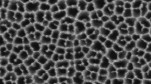
\includegraphics[max size={\textwidth}{\textheight}]{PIL_Test_files/PIL_Test_17_0.jpeg}
    \caption{Элемент исходного изображения}
    \end{subfigure}
    
    \begin{subfigure}{0.325\textwidth}
    \centering
    
\includegraphics[max size={\textwidth}{\textheight}]{PIL_Test_files/PIL_Test_19_0.png}
    \caption{Тот же элемент после установки порога}
    \end{subfigure}
    
    \caption{Установка порога}
 	\end{figure}
   
    \begin{figure}[h]
    \centering
    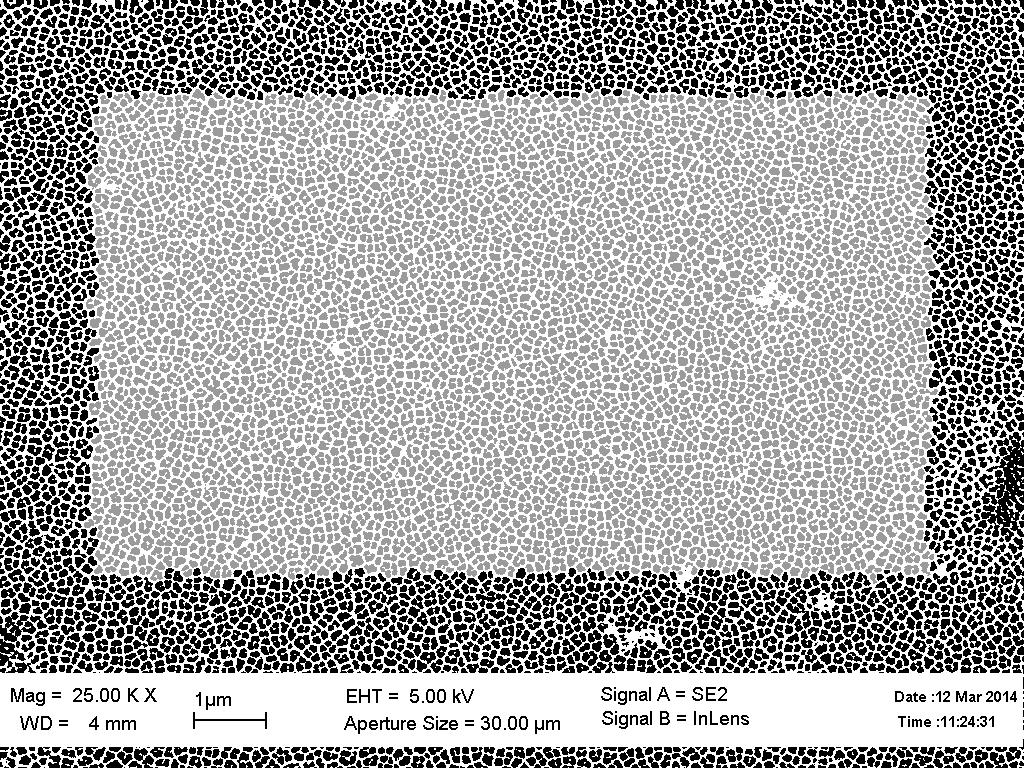
\includegraphics[max size={0.35\textwidth}{\textheight}]{PIL_Test_files/PIL_Test_20_0.jpeg}
    \caption{Результирующее изображение с закрашенными порами}
    \end{figure}
            
        
    
После работы программы остается массив объектов-клеток со всеми
необходимыми данными. Результаты обработки в разделе ``Результаты и
обсуждение''
\subsubsection{Наклоны каналов}
В основе метода для решения данной задачи лежит преобразование Хафа
(Hough Transform). Но предварительная подготовка в этом случае содержит
в себе, кроме описанного выше, использование встроенного в Python Image
Library фильтра поиска границ, иначе алгоритм работал бы неверно. Преобразование Хафа позволяет находить прямые в изображении и получать
значения их параметров. После обработки на входе программы мы имеем
набор черных пикселей, которые имеют значение интенсивности 0, и белых
пикселей, большинство из которых лежат на неидеальных прямых,
коэффициенты наклона которых мы хотим определить. Для любых двух белых
точек картинки мы знаем их координаты в декартовой системе координат:
(X1,Y1) и (X2,Y2). В этом пространстве любая прямая задается двум
коэффициентами: углом наклона A и коэффициентом B, т.е. Y=AX+B. Но если
в новом пространстве в качестве параметров, которыми задается прямая, мы
возьмем не A и B, а X и Y, т.е B=-XA-Y. то в соответствие каждой из двух
точек мы можем поставить по одной прямой в новом пространстве,
называемом пространство Хафа (Hough space). Пересечение этих двух прямых
в пространстве Хафа дает нам точку, координатами которой являются
коэффициенты прямой, на которой лежат две данные точки в исходном
пространстве. После последовательного перебора всех пар точек в
пространстве Хафа мы получим множество прямых и их точек пересечения.
Если нарисовать это множество точек пересечения, причем если для двух
разных пар точка пересечения совпадает, закрашивать ее интенсивнее, то в
итоге мы получим картину, на которой есть локальные максимумы
интенсивности, причем самые яркие точки соответствуют искомым прямым.
Интенсивность этих точек тем больше, чем лучше исходные точки лежат на
одной прямой. Т.к. точки с левой и правой сторон картинки соответствуют
разным прямым, то для оптимизации программы вся картинка разделяется на
несколько частей ширины, в несколько раз превышающей максимальное
расстояние между прямыми на картинке. Также учтено, что преимущественное
направление прямых на фотографии вертикально, поэтому чтобы избежать
обращения коэффициента A в бесконечность, предполагается поворот картины
на 90 градусов. Также в целях оптимизации было решено отсекать те точки
пересечения, которые соответствуют большим углам наклона искомых прямых
(порог выбирается также эмпирически).
Определение края и порога, а также разбиение на части, дали следующие
результаты (Рис. 4)

	\begin{figure}[h]
	\centering
		\begin{subfigure}{0.5\textwidth}
	    	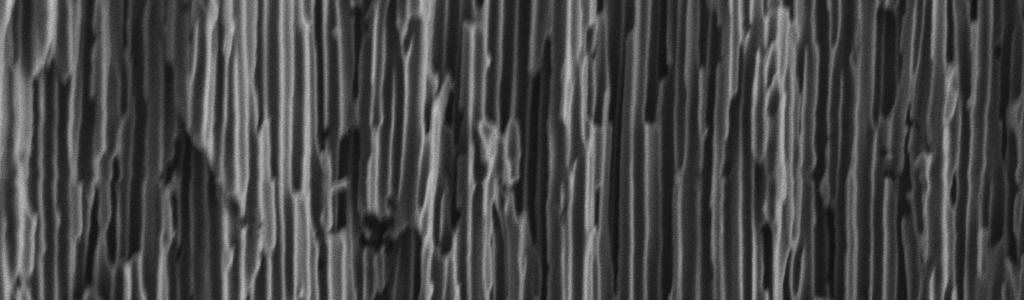
\includegraphics[width = \textwidth]{PIL_Test_files/PIL_Test_26_0.jpeg}
	    \caption{Элемент исходной картинки Рис.1 (с)}
	 	\end{subfigure}
 	
 	\bigskip
    	\begin{subfigure}{0.17\textwidth}
		    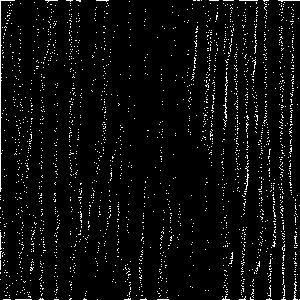
\includegraphics[width=0.9\textwidth]{PIL_Test_files/PIL_Test_27_0.jpeg}
	    \end{subfigure}%~
	    \begin{subfigure}{0.17\textwidth}
	 	   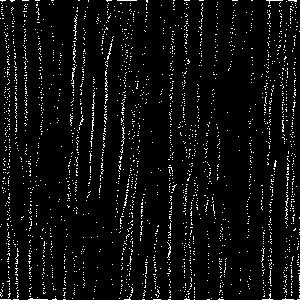
\includegraphics[width = 0.9\textwidth]{PIL_Test_files/PIL_Test_28_0.jpeg}
	    \end{subfigure}%~
	    \begin{subfigure}{0.17\textwidth}
	 	   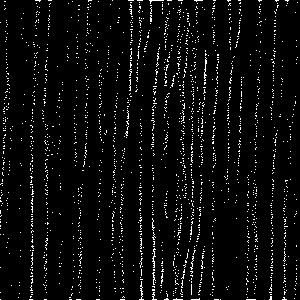
\includegraphics[width = 0.9\textwidth]{PIL_Test_files/PIL_Test_29_0.jpeg}
	    \end{subfigure}
	    \caption{Разбиение (на целое число отрезов заданной ширины) 
	    	и предварительная обработка изображения для Hough transform}
   \end{figure}
        
\FloatBarrier
В пространстве Хафа при анализе второго (среднего) отрезка фотографии
получено следующее распределение интенсивностей:
\FloatBarrier
    \begin{figure*}
    \centering
    	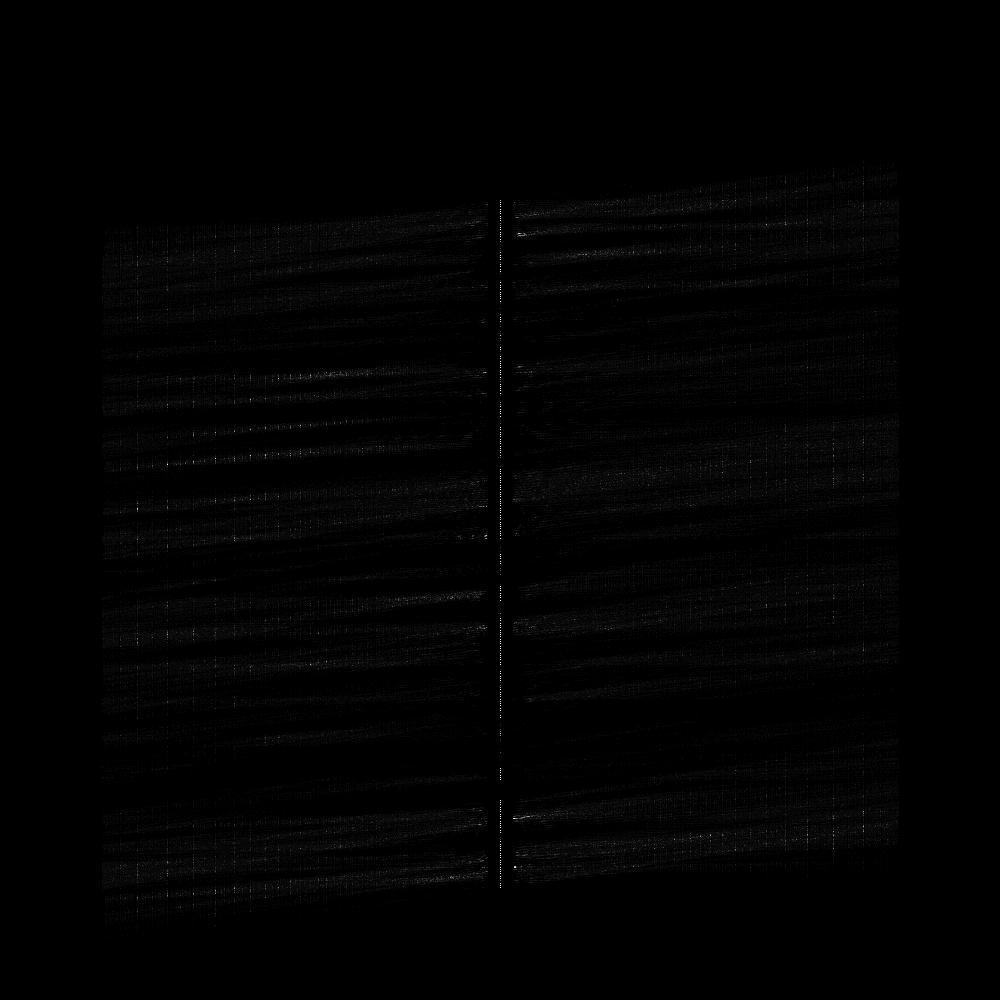
\includegraphics[max size={\textwidth}{\textheight}]{PIL_Test_files/PIL_Test_31_0.jpeg}
    	\caption{Распределение интенсивностей в пространстве Хафа}
    \end{figure*}
\FloatBarrier
    

    \begin{figure*}
    \begin{subfigure}{\textwidth}
    \centering
    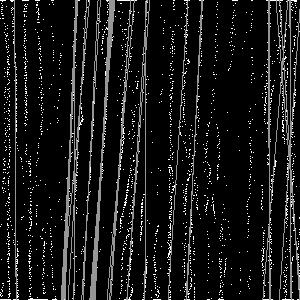
\includegraphics[max size={0.3\textwidth}{\textheight}]{PIL_Test_files/PIL_Test_33_0.jpeg}
    \caption{Обнаруженные прямые на обработанной части изображения}
    \end{subfigure}
    
    \begin{subfigure}{\textwidth}
    \centering
    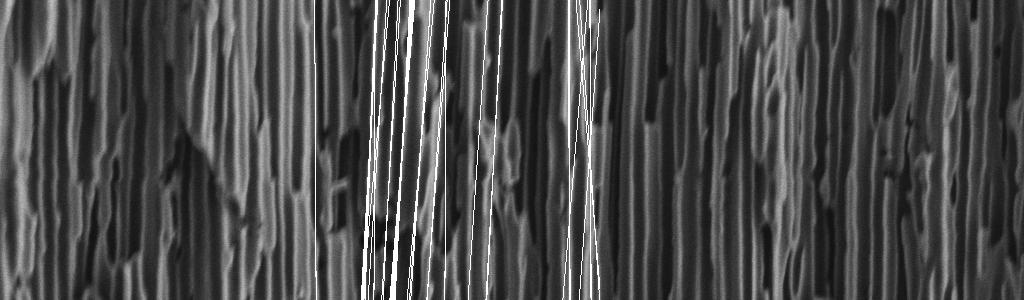
\includegraphics[max size={\textwidth}{\textheight}]{PIL_Test_files/PIL_Test_35_0.jpeg}
    \caption{Обнаруженные прямые на оригинале}
    \end{subfigure}
    \caption{Демонстрация обнаружения прямых}
    \end{figure*}
        
    \FloatBarrier
 
Это распределение позволило определить на фотографии следующие прямые - Рис. 6.

Коэффициенты всех обнаруженных прямых после работы программы сохраняются
в памяти компьютера, поэтому возможна любая дальнейшая статистическая
обработка.
\FloatBarrier
\section{Результаты и обсуждение}



\subsection{Размеры пор}
    \begin{figure}[h]
    \begin{subfigure}{0.45\textwidth}
    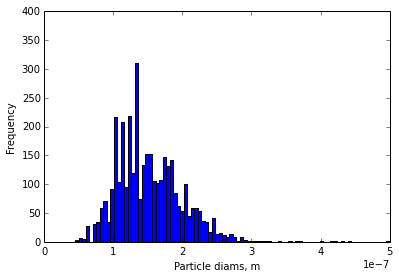
\includegraphics[max size={\textwidth}{\textheight}]{PIL_Test_files/index.png}
    \end{subfigure}
    
    \begin{subfigure}{0.45\textwidth}
    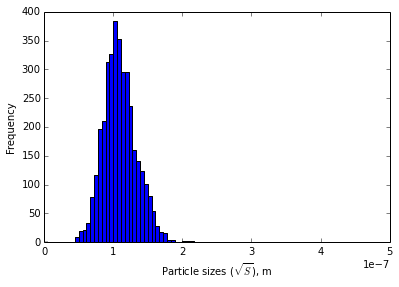
\includegraphics[max size={\textwidth}{\textheight}]{PIL_Test_files/index1.png}
    \end{subfigure}
    
    \caption{Гистограммы распределения пор по размерам (для первой и второй нормы клеток)}
    \end{figure}
    
В результате анализа данных были получены: гистограмма распределения
размеров пор (Рис. 7), усредненные размеры пор двумя способами (корень из площади
и диаметр), характерное отклонение от цилиндричности по разности
вычисленных характерных средних размеров, плотность пор.


Заявленный средний размер хорошо совпадает с рассчитанным -
$0.11 \pm 0.05$ мкм. В тоже время в плотности пор обнаружены
существенные расхождения: заявленное значение в $2\cdot 10^8$ см$^{-2}$
отличается от вычисленного $4\cdot 10^9$ см$^{-2}$ в 20 раз. Характерное
отклонение от цилиндричности составило $-2.85\cdot 10^{-8}$ мкм, то есть
в среднем преобладает вытянутая форма пор (поры вытянуты на 29\%).


\subsection{Толщина мембраны}
Измеренная толщина мембраны составила 57 мкм, что почти в три раза
отличается от заявленной 22 мкм.
\subsection{Каналы}
По результатам работы программы получено среднее по модулю отклонение от
вертикали в 2$^\circ$ в толще мембраны.Имеется также тенденция к
искривлению каналов относительно прямых линий. О количестве дефектов
сложно судить в силу наличия большого количества механических
повреждений на сколе.
\subsection{Выводы}
Имеются существенные отклонения от заявленных параметров. Разницу в толщине больше чем в два раза можно объяснить тем, что, скорее всего, исследовался фильтр другой модели с иными параметрами. Тем же может быть объяснена и разница в плотности, хотя для этого параметра возможна вариация от одной стороны мембраны к другой даже в пределах одной модели. Второе могло бы быть важно в свете того, что в данной работе исследовалась только одна сторона, соответствующая Рис.1 (а), но с другой стороны, различие плотности пор в 20 раз означало бы, что, начавшись на одной стороне, 20 пор, в среднем, срастались бы в одну на другой стороне, что маловероятно, так как для фильтра важна пропускная способность.

Мембрана, скорее всего, непригодна для выращивания нанопроводов.
Качество каналов как и в плане цилиндричности, так и в плане постоянства
наклона, недостаточно, на наш взгляд, для формирования проводов длины,
сравнимой с толщиной пластины.
\section{Приложение}
Здесь представлены процедуры работы с программами, написанными нами. Исодный код можно найти по адресу https://github.com/vdrhtc/CellDistinguisher
\subsection{Cell distinguisher}

    % Make sure that atleast 4 lines are below the HR
    \needspace{4\baselineskip}

    
        \vspace{6pt}
        \makebox[0.1\linewidth]{\smaller\hfill\tt\color{nbframe-in-prompt}In\hspace{4pt}{[}1{]}:\hspace{4pt}}\\*
        \vspace{-2\baselineskip}
        \begin{ColorVerbatim}
            \vspace{-0\baselineskip}
            \begin{Verbatim}[commandchars=\\\{\}]
\PY{o}{\PYZpc{}}\PY{k}{pylab} \PY{n}{inline}
\PY{k+kn}{import} \PY{n+nn}{sys}
\PY{n}{sys}\PY{o}{.}\PY{n}{path}\PY{o}{.}\PY{n}{append}\PY{p}{(}\PY{l+s}{\PYZsq{}}\PY{l+s}{src}\PY{l+s}{\PYZsq{}}\PY{p}{)}
\PY{k+kn}{from} \PY{n+nn}{PIL} \PY{k+kn}{import} \PY{n}{Image}\PY{p}{,} \PY{n}{ImageFilter}
\PY{k+kn}{from} \PY{n+nn}{cell\PYZus{}distinguisher.distinguisher} \PY{k+kn}{import} \PY{o}{*}
\PY{k+kn}{from} \PY{n+nn}{line\PYZus{}distinguisher.distinguisher} \PY{k+kn}{import} \PY{o}{*}
\end{Verbatim}

            
                \vspace{-0.2\baselineskip}
            
        \end{ColorVerbatim}
    

    

        % If the first block is an image, minipage the image.  Else
        % request a certain amount of space for the input text.
        \needspace{4\baselineskip}
        
        

            % Add document contents.
            
                \begin{InvisibleVerbatim}
                \vspace{-0\baselineskip}
\begin{alltt}Populating the interactive namespace from numpy and matplotlib
\end{alltt}

            \end{InvisibleVerbatim}
            
        
    


    % Make sure that atleast 4 lines are below the HR
    \needspace{4\baselineskip}

    
        \vspace{6pt}
        \makebox[0.1\linewidth]{\smaller\hfill\tt\color{nbframe-in-prompt}In\hspace{4pt}{[}2{]}:\hspace{4pt}}\\*
        \vspace{-2\baselineskip}
        \begin{ColorVerbatim}
            \vspace{-0\baselineskip}
            \begin{Verbatim}[commandchars=\\\{\}]
\PY{n}{pixel\PYZus{}size} \PY{o}{=} \PY{l+m+mf}{1e\PYZhy{}6}\PY{o}{/}\PY{l+m+mi}{70}
\end{Verbatim}

            
                \vspace{-0.2\baselineskip}
            
        \end{ColorVerbatim}
    


    % Make sure that atleast 4 lines are below the HR
    \needspace{4\baselineskip}

    
        \vspace{6pt}
        \makebox[0.1\linewidth]{\smaller\hfill\tt\color{nbframe-in-prompt}In\hspace{4pt}{[}3{]}:\hspace{4pt}}\\*
        \vspace{-2\baselineskip}
        \begin{ColorVerbatim}
            \vspace{-0\baselineskip}
            \begin{Verbatim}[commandchars=\\\{\}]
\PY{n}{im} \PY{o}{=} \PY{n}{Image}\PY{o}{.}\PY{n}{open}\PY{p}{(}\PY{l+s}{\PYZsq{}}\PY{l+s}{1\PYZus{}01.tif}\PY{l+s}{\PYZsq{}}\PY{p}{)}
\PY{n}{im}\PY{o}{.}\PY{n}{show}\PY{p}{(}\PY{p}{)}
\end{Verbatim}

            
                \vspace{-0.2\baselineskip}
            
        \end{ColorVerbatim}
    


    % Make sure that atleast 4 lines are below the HR
    \needspace{4\baselineskip}

    
        \vspace{6pt}
        \makebox[0.1\linewidth]{\smaller\hfill\tt\color{nbframe-in-prompt}In\hspace{4pt}{[}4{]}:\hspace{4pt}}\\*
        \vspace{-2\baselineskip}
        \begin{ColorVerbatim}
            \vspace{-0\baselineskip}
            \begin{Verbatim}[commandchars=\\\{\}]
\PY{n}{altered\PYZus{}im} \PY{o}{=} \PY{n}{get\PYZus{}cells\PYZus{}from\PYZus{}image}\PY{p}{(}\PY{n}{im}\PY{p}{,} \PY{p}{(}\PY{l+m+mi}{100}\PY{p}{,} \\ \PY{l+m+mi}{100}\PY{p}{)} \PY{p}{,} \PY{p}{(}\PY{n}{im}\PY{o}{.}\PY{n}{getbbox}\PY{p}{(}\PY{p}{)}\PY{p}{[}\PY{l+m+mi}{2}\PY{p}{]}\PY{o}{\PYZhy{}}\PY{l+m+mi}{100}\PY{p}{,} \PY{n}{im}\PY{o}{.}\PY{n}{getbbox}\PY{p}{(}\PY{p}{)}\PY{p}{[}\PY{l+m+mi}{3}\PY{p}{]}\PY{o}{\PYZhy{}}\PY{l+m+mi}{200}\PY{p}{)}\PY{p}{,} \PY{n}{pixel\PYZus{}size}\PY{p}{,} \PY{l+m+mi}{80}\PY{p}{)}
\end{Verbatim}

            
                \vspace{-0.2\baselineskip}
            
        \end{ColorVerbatim}
    


    % Make sure that atleast 4 lines are below the HR
    \needspace{4\baselineskip}

    
        \vspace{6pt}
        \makebox[0.1\linewidth]{\smaller\hfill\tt\color{nbframe-in-prompt}In\hspace{4pt}{[}143{]}:\hspace{4pt}}\\*
        \vspace{-2\baselineskip}
        \begin{ColorVerbatim}
            \vspace{-0\baselineskip}
            \begin{Verbatim}[commandchars=\\\{\}]
\PY{n}{altered\PYZus{}im}\PY{o}{.}\PY{n}{show}\PY{p}{(}\PY{p}{)}
\end{Verbatim}

            
                \vspace{-0.2\baselineskip}
            
        \end{ColorVerbatim}
    


    % Make sure that atleast 4 lines are below the HR
    \needspace{4\baselineskip}

    
        \vspace{6pt}
        \makebox[0.1\linewidth]{\smaller\hfill\tt\color{nbframe-in-prompt}In\hspace{4pt}{[}5{]}:\hspace{4pt}}\\*
        \vspace{-2\baselineskip}
        \begin{ColorVerbatim}
            \vspace{-0\baselineskip}
            \begin{Verbatim}[commandchars=\\\{\}]
\PY{n+nb}{len}\PY{p}{(}\PY{n}{cells}\PY{p}{)}
\end{Verbatim}

            
                \vspace{-0.2\baselineskip}
            
        \end{ColorVerbatim}
    

    

        % If the first block is an image, minipage the image.  Else
        % request a certain amount of space for the input text.
        \needspace{4\baselineskip}
        
        

            % Add document contents.
            
                \makebox[0.1\linewidth]{\smaller\hfill\tt\color{nbframe-out-prompt}Out\hspace{4pt}{[}5{]}:\hspace{4pt}}\\*
                \vspace{-2\baselineskip}\begin{InvisibleVerbatim}
                \vspace{-0\baselineskip}
\begin{alltt}3626\end{alltt}

            \end{InvisibleVerbatim}
            
        
    


    % Make sure that atleast 4 lines are below the HR
    \needspace{4\baselineskip}

    
        \vspace{6pt}
        \makebox[0.1\linewidth]{\smaller\hfill\tt\color{nbframe-in-prompt}In\hspace{4pt}{[}11{]}:\hspace{4pt}}\\*
        \vspace{-2\baselineskip}
        \begin{ColorVerbatim}
            \vspace{-0\baselineskip}
            \begin{Verbatim}[commandchars=\\\{\}]
\PY{n}{sizes} \PY{o}{=} \PY{p}{[}\PY{n}{cell}\PY{o}{.}\PY{n}{first\PYZus{}norm}\PY{p}{(}\PY{p}{)} \PY{k}{for} \PY{n}{cell} \PY{o+ow}{in} \PY{n}{cells}\PY{p}{]}
\PY{n}{sizes1} \PY{o}{=} \PY{p}{[}\PY{n}{cell}\PY{o}{.}\PY{n}{second\PYZus{}norm}\PY{p}{(}\PY{p}{)} \PY{k}{for} \PY{n}{cell} \PY{o+ow}{in} \PY{n}{cells}\PY{p}{]} 
\PY{n}{deltas} \PY{o}{=} \PY{n+nb}{map}\PY{p}{(}\PY{k}{lambda} \PY{n}{x}\PY{p}{,} \PY{n}{y}\PY{p}{:} \PY{n}{x}\PY{o}{*}\PY{n}{math}\PY{o}{.}\PY{n}{sqrt}\PY{p}{(}\PY{l+m+mi}{4}\PY{o}{/}\PY{n}{math}\PY{o}{.}\PY{n}{pi}\PY{p}{)}\PY{o}{\PYZhy{}}\PY{n}{y}\PY{p}{,} \PY{n}{sizes}\PY{p}{,} \PY{n}{sizes1}\PY{p}{)}
\end{Verbatim}

            
                \vspace{-0.2\baselineskip}
            
        \end{ColorVerbatim}
    


    % Make sure that atleast 4 lines are below the HR
    \needspace{4\baselineskip}

    
        \vspace{6pt}
        \makebox[0.1\linewidth]{\smaller\hfill\tt\color{nbframe-in-prompt}In\hspace{4pt}{[}13{]}:\hspace{4pt}}\\*
        \vspace{-2\baselineskip}
        \begin{ColorVerbatim}
            \vspace{-0\baselineskip}
            \begin{Verbatim}[commandchars=\\\{\}]
\PY{n}{plt}\PY{o}{.}\PY{n}{hist}\PY{p}{(}\PY{n}{sizes}\PY{p}{,} \PY{l+m+mi}{50}\PY{p}{)}
\PY{k}{print}\PY{p}{(}\PY{l+s}{\PYZdq{}}\PY{l+s}{Средний рамер поры по корню из площади: }\PY{l+s+si}{\PYZpc{}.2e}\PY{l+s}{\PYZdq{}}\PY{o}{\PYZpc{}} \PY{n}{mean}\PY{p}{(}\PY{n}{sizes}\PY{p}{)}\PY{p}{)}
\PY{k}{print}\PY{p}{(}\PY{l+s}{\PYZdq{}}\PY{l+s}{Средний рамер поры по диаметру: }\PY{l+s+si}{\PYZpc{}.2e}\PY{l+s}{\PYZdq{}}\PY{o}{\PYZpc{}} \PY{n}{mean}\PY{p}{(}\PY{n}{sizes1}\PY{p}{)}\PY{p}{)}
\PY{k}{print}\PY{p}{(}\PY{l+s}{\PYZdq{}}\PY{l+s}{Среднее отклонение от цилиндричности: }\PY{l+s+si}{\PYZpc{}.2e}\PY{l+s}{\PYZdq{}}\PY{o}{\PYZpc{}} \PY{n}{mean}\PY{p}{(}\PY{n+nb}{list}\PY{p}{(}\PY{n}{deltas}\PY{p}{)}\PY{p}{)}\PY{p}{)}
\PY{k}{print}\PY{p}{(}\PY{l+s}{\PYZdq{}}\PY{l+s}{Плотность пор: }\PY{l+s+si}{\PYZpc{}.2e}\PY{l+s}{\PYZdq{}}\PY{o}{\PYZpc{}}\PY{p}{(}\PY{n+nb}{len}\PY{p}{(}\PY{n}{cells}\PY{p}{)}\PY{o}{/}\PY{p}{(}\PY{p}{(}\PY{n}{im}\PY{o}{.} \\ \PY{n}{getbbox}\PY{p}{(}\PY{p}{)}\PY{p}{[}\PY{l+m+mi}{2}\PY{p}{]}\PY{o}{\PYZhy{}}\PY{l+m+mi}{200}\PY{p}{)}\PY{o}{*}\PY{p}{(} \\ \PY{n}{im}\PY{o}{.}\PY{n}{getbbox}\PY{p}{(}\PY{p}{)}\PY{p}{[}\PY{l+m+mi}{3}\PY{p}{]}\PY{o}{\PYZhy{}}\PY{l+m+mi}{300}\PY{p}{)}\PY{o}{*}\PY{p}{(}\PY{n}{pixel\PYZus{}size}\PY{o}{*}\PY{l+m+mi}{100}\PY{p}{)}\PY{o}{*}\PY{o}{*}\PY{l+m+mi}{2}\PY{p}{)}\PY{p}{)}\PY{p}{)}
\end{Verbatim}

            
                \vspace{-0.2\baselineskip}
            
        \end{ColorVerbatim}
    

    

        % If the first block is an image, minipage the image.  Else
        % request a certain amount of space for the input text.
        \needspace{4\baselineskip}
        
        

            % Add document contents.
            
                \begin{InvisibleVerbatim}
                \vspace{-0\baselineskip}
\begin{alltt}Средний рамер поры по корню из площади: 1.09e-07
Средний рамер поры по диаметру: 1.52e-07
Среднее отклонение от цилиндричности: -2.85e-08
Плотность пор: 4.61e+09
\end{alltt}

            \end{InvisibleVerbatim}
            
                \begin{InvisibleVerbatim}
                \vspace{-0\baselineskip}
    \begin{center}
    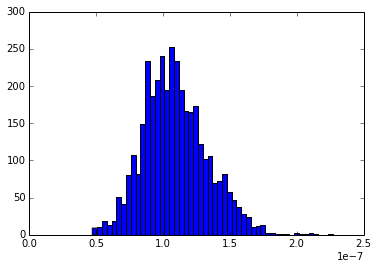
\includegraphics[max size={\textwidth}{\textheight}]{PIL_Test_files/PIL_Test_57_1.png}
    \par
    \end{center}
    
            \end{InvisibleVerbatim}
            
        
    


    % Make sure that atleast 4 lines are below the HR
    \needspace{4\baselineskip}

    
        \vspace{6pt}
        \makebox[0.1\linewidth]{\smaller\hfill\tt\color{nbframe-in-prompt}In\hspace{4pt}{[}124{]}:\hspace{4pt}}\\*
        \vspace{-2\baselineskip}
        \begin{ColorVerbatim}
            \vspace{-0.7\baselineskip}
            \begin{Verbatim}[commandchars=\\\{\}]
\PY{k+kn}{import} \PY{n+nn}{sys}
\PY{n}{sys}\PY{o}{.}\PY{n}{path}\PY{o}{.}\PY{n}{append}\PY{p}{(}\PY{l+s}{\PYZsq{}}\PY{l+s}{src}\PY{l+s}{\PYZsq{}}\PY{p}{)}
\PY{k+kn}{from} \PY{n+nn}{PIL} \PY{k+kn}{import} \PY{n}{Image}\PY{p}{,} \PY{n}{ImageFilter}
\PY{k+kn}{from} \PY{n+nn}{cell\PYZus{}distinguisher.distinguisher} \PY{k+kn}{import} \PY{o}{*}
\PY{k+kn}{from} \PY{n+nn}{line\PYZus{}distinguisher.distinguisher} \PY{k+kn}{import} \PY{o}{*}
\PY{o}{\PYZpc{}}\PY{k}{pylab} \PY{n}{inline}
\end{Verbatim}

            
                \vspace{-0.2\baselineskip}
            
        \end{ColorVerbatim}
    

    

        % If the first block is an image, minipage the image.  Else
        % request a certain amount of space for the input text.
        \needspace{4\baselineskip}
        
        

            % Add document contents.
            
            
              
            
        
    
\subsection{Line distinguisher}

    % Make sure that atleast 4 lines are below the HR
    \needspace{4\baselineskip}

    
        \vspace{6pt}
        \makebox[0.1\linewidth]{\smaller\hfill\tt\color{nbframe-in-prompt}In\hspace{4pt}{[}133{]}:\hspace{4pt}}\\*
        \vspace{-2\baselineskip}
        \begin{ColorVerbatim}
            \vspace{-0\baselineskip}
            \begin{Verbatim}[commandchars=\\\{\}]
\PY{n}{im1} \PY{o}{=} \PY{n}{Image}\PY{o}{.}\PY{n}{open}\PY{p}{(}\PY{l+s}{\PYZsq{}}\PY{l+s}{./1\PYZus{}10.tif}\PY{l+s}{\PYZsq{}}\PY{p}{)}\PY{o}{.} \\ \PY{n}{crop}\PY{p}{(}\PY{p}{(}\PY{l+m+mi}{0}\PY{p}{,} \PY{l+m+mi}{300}\PY{p}{,} \PY{l+m+mi}{1024}\PY{p}{,} \PY{l+m+mi}{600}\PY{p}{)}\PY{p}{)}
\PY{n}{im1}\PY{o}{.}\PY{n}{show}\PY{p}{(}\PY{p}{)}
\end{Verbatim}

            
                \vspace{-0.2\baselineskip}
            
        \end{ColorVerbatim}
    


    % Make sure that atleast 4 lines are below the HR
    \needspace{4\baselineskip}

    
        \vspace{6pt}
        \makebox[0.1\linewidth]{\smaller\hfill\tt\color{nbframe-in-prompt}In\hspace{4pt}{[}47{]}:\hspace{4pt}}\\*
        \vspace{-2\baselineskip}
        \begin{ColorVerbatim}
            \vspace{-0\baselineskip}
            \begin{Verbatim}[commandchars=\\\{\}]
\PY{n}{slices} \PY{o}{=} \PY{n}{prepare\PYZus{}image}\PY{p}{(}\PY{n}{im1}\PY{p}{,} \PY{n}{threshold}\PY{o}{=}\PY{l+m+mi}{80}\PY{p}{,} \\ \PY{n}{slice\PYZus{}thickness}\PY{o}{=}\PY{l+m+mi}{300}\PY{p}{)}
\end{Verbatim}

            
                \vspace{-0.2\baselineskip}
            
        \end{ColorVerbatim}
    


    % Make sure that atleast 4 lines are below the HR
    \needspace{4\baselineskip}

    
        \vspace{6pt}
        \makebox[0.1\linewidth]{\smaller\hfill\tt\color{nbframe-in-prompt}In\hspace{4pt}{[}56{]}:\hspace{4pt}}\\*
        \vspace{-2\baselineskip}
        \begin{ColorVerbatim}
            \vspace{-0\baselineskip}
            \begin{Verbatim}[commandchars=\\\{\}]
\PY{n}{slices}\PY{p}{[}\PY{l+m+mi}{2}\PY{p}{]}\PY{o}{.}\PY{n}{show}\PY{p}{(}\PY{p}{)}
\end{Verbatim}

            
                \vspace{-0.2\baselineskip}
            
        \end{ColorVerbatim}
    


    % Make sure that atleast 4 lines are below the HR
    \needspace{4\baselineskip}

    
        \vspace{6pt}
        \makebox[0.1\linewidth]{\smaller\hfill\tt\color{nbframe-in-prompt}In\hspace{4pt}{[}67{]}:\hspace{4pt}}\\*
        \vspace{-2\baselineskip}
        \begin{ColorVerbatim}
            \vspace{-0\baselineskip}
            \begin{Verbatim}[commandchars=\\\{\}]
\PY{n}{coeffs} \PY{o}{=} \PY{n}{get\PYZus{}lines}\PY{p}{(}\PY{n}{slices}\PY{p}{[}\PY{l+m+mi}{1}\PY{p}{]}\PY{p}{,} \PY{n}{tolerance\PYZus{}a\PYZus{}b}\PY{o}{=}\PY{p}{(}\PY{l+m+mi}{4}\PY{p}{,} \PY{l+m+mi}{1}\PY{p}{)}\PY{p}{,} \\ \PY{n}{max\PYZus{}a}\PY{o}{=}\PY{l+m+mf}{0.1}\PY{p}{)}
\end{Verbatim}

            
                \vspace{-0.2\baselineskip}
            
        \end{ColorVerbatim}
    

    

        % If the first block is an image, minipage the image.  Else
        % request a certain amount of space for the input text.
        \needspace{4\baselineskip}
        
        

            % Add document contents.
            
                \begin{InvisibleVerbatim}
                \vspace{-0\baselineskip}
\begin{alltt}Getting coefficients\ldots
Processing  4575 points.
485186, 4574
\end{alltt}

            \end{InvisibleVerbatim}
            
        
    


    % Make sure that atleast 4 lines are below the HR
    \needspace{4\baselineskip}

    
        \vspace{6pt}
        \makebox[0.1\linewidth]{\smaller\hfill\tt\color{nbframe-in-prompt}In\hspace{4pt}{[}68{]}:\hspace{4pt}}\\*
        \vspace{-2\baselineskip}
        \begin{ColorVerbatim}
            \vspace{-0\baselineskip}
            \begin{Verbatim}[commandchars=\\\{\}]
\PY{n}{max\PYZus{}coeff} \PY{o}{=} \PY{n+nb}{max}\PY{p}{(}\PY{n+nb}{list}\PY{p}{(}\PY{n}{coeffs}\PY{o}{.}\PY{n}{values}\PY{p}{(}\PY{p}{)}\PY{p}{)}\PY{p}{)}
\end{Verbatim}

            
                \vspace{-0.2\baselineskip}
            
        \end{ColorVerbatim}
    


    % Make sure that atleast 4 lines are below the HR
    \needspace{4\baselineskip}

    
        \vspace{6pt}
        \makebox[0.1\linewidth]{\smaller\hfill\tt\color{nbframe-in-prompt}In\hspace{4pt}{[}109{]}:\hspace{4pt}}\\*
        \vspace{-2\baselineskip}
        \begin{ColorVerbatim}
            \vspace{-0\baselineskip}
            \begin{Verbatim}[commandchars=\\\{\}]
\PY{n}{image} \PY{o}{=} \PY{n}{Image}\PY{o}{.}\PY{n}{new}\PY{p}{(}\PY{l+s}{\PYZdq{}}\PY{l+s}{L}\PY{l+s}{\PYZdq{}}\PY{p}{,} \PY{p}{(}\PY{l+m+mi}{1000}\PY{p}{,} \PY{l+m+mi}{1000}\PY{p}{)}\PY{p}{)}
\PY{n}{interesting\PYZus{}points} \PY{o}{=} \PY{p}{[}\PY{p}{]}

\PY{n}{column} \PY{o}{=} \PY{l+m+mi}{0}
\PY{k}{for} \PY{n}{point} \PY{o+ow}{in} \PY{n}{coeffs}\PY{o}{.}\PY{n}{keys}\PY{p}{(}\PY{p}{)}\PY{p}{:}
    \PY{n}{level} \PY{o}{=} \PY{n}{max\PYZus{}coeff}
    
    \PY{k}{if} \PY{n}{coeffs}\PY{p}{[}\PY{n}{point}\PY{p}{]} \PY{o}{\PYZgt{}} \PY{n}{max\PYZus{}coeff}\PY{o}{/}\PY{l+m+mi}{130} \PY{o+ow}{and} \PY{n}{point}\PY{p}{[}\PY{l+m+mi}{0}\PY{p}{]}\PY{o}{!=}\PY{l+m+mi}{0}\PY{p}{:}
        \PY{n}{interesting\PYZus{}points}\PY{o}{.}\PY{n}{append}\PY{p}{(}\PY{n}{point}\PY{p}{)}
        
        \PY{k}{if} \PY{n}{column} \PY{o}{!=} \PY{l+m+mi}{2}\PY{p}{:}
            \PY{k}{print}\PY{p}{(}\PY{n}{point}\PY{p}{,} \PY{n}{end} \PY{o}{=} \PY{l+s}{\PYZsq{}}\PY{l+s}{       }\PY{l+s}{\PYZsq{}}\PY{p}{)}
            \PY{n}{column}\PY{o}{+}\PY{o}{=}\PY{l+m+mi}{1}
        \PY{k}{else}\PY{p}{:}
            \PY{k}{print}\PY{p}{(}\PY{n}{point}\PY{p}{)}
            \PY{n}{column} \PY{o}{=} \PY{l+m+mi}{0}
            
    \PY{n}{image}\PY{o}{.}\PY{n}{putpixel}\PY{p}{(}\PY{p}{(}\PY{n+nb}{int}\PY{p}{(}\PY{n}{point}\PY{p}{[}\PY{l+m+mi}{0}\PY{p}{]}\PY{o}{*}\PY{l+m+mf}{4e3}\PY{p}{)}\PY{o}{+}\PY{l+m+mi}{500}\PY{p}{,} \PY{n+nb}{int}\PY{p}{(} \\ \PY{n}{point}\PY{p}{[}\PY{l+m+mi}{1}\PY{p}{]}\PY{o}{*}\PY{l+m+mf}{2.3}\PY{p}{)}\PY{o}{+}\PY{l+m+mi}{200}\PY{p}{)}\PY{p}{,} \\ \PY{n+nb}{int}\PY{p}{(}\PY{n}{coeffs}\PY{p}{[} \PY{n}{point}\PY{p}{]}\PY{o}{/}\PY{n}{level}\PY{o}{*}\PY{l+m+mi}{255}\PY{o}{*}\PY{l+m+mi}{90}\PY{p}{)}\PY{p}{)}
\PY{c}{\PYZsh{} image.show()}
\end{Verbatim}

            
                \vspace{-0.2\baselineskip}
            
        \end{ColorVerbatim}
    

    

        % If the first block is an image, minipage the image.  Else
        % request a certain amount of space for the input text.
        \needspace{4\baselineskip}
        
        

            % Add document contents.
            
                \begin{InvisibleVerbatim}
                \vspace{-0\baselineskip}
\begin{alltt}
(-0.0625, 111.6)       (0.0037, 268.9)          (-0.0714, 300.6)
(-0.0833, 287.8)       (-0.05, 77.5)          (-0.0036, 146.0)
(0.0039, 268.9)       (0.0068, 268.0          (-0.0417, 76.1)
(-0.0714, 113.4)       (-0.0667, 130.7)          (0.0038, 290.0)
(0.0035, 290.0)       (-0.0667, 188.0)          (-0.04, 75.8)
(-0.0667, 147.1)       (0.0667, 279.7)         (-0.0714, 130.9)
(-0.0769, 149.8)       (-0.0038, 75.1)         (-0.0039, 75.1)
(-0.0667, 112.5)       (0.0041, 268.9)         (-0.0455, 76.9)
(-0.0435, 76.5)       (-0.0909, 89.5)         (-0.0435, 77.0)
(-0.05, 77.0)       (-0.0455, 76.7)         (-0.0714, 113.1)
(-0.0476, 76.8)       (-0.05, 201.7)         (-0.05, 110.0)
(-0.0455, 76.4)       (-0.0357, 75.7)         (-0.0526, 77.5)
(0.004, 289.9)       (-0.0714, 112.9)         (0.0036, 268.9)
(-0.0556, 110.7)       (0.0037, 289.9)         (-0.0909, 134.2)
(-0.05, 109.8)       (0.0035, 269.0)         (0.0833, 276.0)
(-0.0769, 113.8)       (-0.0588, 110.9)         (-0.0417, 75.8)
(-0.0417, 76.2)       (-0.0037, 146.0)         (-0.0625, 100.4)
(0.0034, 269.0)       (-0.05, 77.2)         (-0.0625, 86.8)
(0.004, 268.9)       (-0.0833, 114.8)         (-0.0556, 77.8)
(0.0039, 289.9)       (0.0047, 14.7)         (0.0036, 269.0)
(0.0048, 14.7)       (0.0038, 268.9)         (0.0037, 290.0)
(-0.0556, 202.6)       (0.0037, 269.0)         (-0.05, 98.0)
(0.0036, 290.0)       (0.0038, 289.9)         (-0.0625, 111.3)
(-0.0714, 112.6)
\end{alltt}

            \end{InvisibleVerbatim}
            
        
    


    % Make sure that atleast 4 lines are below the HR
    \needspace{4\baselineskip}

    
        \vspace{6pt}
        \makebox[0.1\linewidth]{\smaller\hfill\tt\color{nbframe-in-prompt}In\hspace{4pt}{[}117{]}:\hspace{4pt}}\\*
        \vspace{-2\baselineskip}
        \begin{ColorVerbatim}
            \vspace{-0\baselineskip}
            \begin{Verbatim}[commandchars=\\\{\}]
\PY{n}{copy} \PY{o}{=} \PY{n}{slices}\PY{p}{[}\PY{l+m+mi}{1}\PY{p}{]}\PY{o}{.}\PY{n}{copy}\PY{p}{(}\PY{p}{)}
\end{Verbatim}

            
                \vspace{-0.2\baselineskip}
            
        \end{ColorVerbatim}
    


    % Make sure that atleast 4 lines are below the HR
    \needspace{4\baselineskip}

    
        \vspace{6pt}
        \makebox[0.1\linewidth]{\smaller\hfill\tt\color{nbframe-in-prompt}In\hspace{4pt}{[}113{]}:\hspace{4pt}}\\*
        \vspace{-2\baselineskip}
        \begin{ColorVerbatim}
            \vspace{-0\baselineskip}
            \begin{Verbatim}[commandchars=\\\{\}]
\PY{k}{for} \PY{n}{interesting\PYZus{}point} \PY{o+ow}{in} \PY{n}{interesting\PYZus{}points}\PY{p}{:}
    \PY{k}{for} \PY{n}{y} \PY{o+ow}{in} \PY{n+nb}{range}\PY{p}{(}\PY{l+m+mi}{0}\PY{p}{,} \PY{n}{copy}\PY{o}{.}\PY{n}{getbbox}\PY{p}{(}\PY{p}{)}\PY{p}{[} \PY{l+m+mi}{3}\PY{p}{]}\PY{p}{)}\PY{p}{:}
\PY{c}{\PYZsh{}         print(interesting\PYZus{}point, int(interesting \\ \PYZus{}point[0]*y+interesting\PYZus{}point[1]), y)} 
        \PY{k}{if} \PY{n+nb}{int}\PY{p}{(}\PY{n}{interesting\PYZus{}point}\PY{p}{[}\PY{l+m+mi}{0}\PY{p}{]}\PY{o}{*}\PY{n}{y} \\ \PY{o}{+}\PY{n}{interesting\PYZus{}point}\PY{p}{[}\PY{l+m+mi}{1}\PY{p}{]}\PY{p}{)} \PY{o}{\PYZgt{}} \PY{l+m+mi}{0} \PY{o+ow}{and} \newline \PY{n+nb}{int}\PY{p}{(}\PY{n}{interesting\PYZus{}point}\PY{p}{[}\PY{l+m+mi}{0}\PY{p}{]}\PY{o}{*} \\ \PY{n}{y}\PY{o}{+}\PY{n}{interesting\PYZus{}point}\PY{p}{[}\PY{l+m+mi}{1}\PY{p}{]}\PY{p}{)} \PY{o}{\PYZlt{}} \PY{n}{copy}\PY{o}{.}\PY{n}{getbbox}\PY{p}{(}\PY{p}{)}\PY{p}{[}\PY{l+m+mi}{2}\PY{p}{]}\PY{p}{:}
            \PY{n}{copy}\PY{o}{.}\PY{n}{putpixel}\PY{p}{(}\PY{p}{(}\PY{n+nb}{int}\PY{p}{(}\PY{n}{interesting\PYZus{}point}\PY{p}{[}\PY{l+m+mi}{0}\PY{p}{]}\PY{o}{*}\PY{n}{y}\PY{o}{+} \\ \PY{n}{interesting\PYZus{}point}\PY{p}{[}\PY{l+m+mi}{1}\PY{p}{]}\PY{p}{)}\PY{p}{,} \PY{n}{y}\PY{p}{)}\PY{p}{,} \PY{l+m+mi}{150}\PY{p}{)}
\PY{n}{copy}\PY{o}{.}\PY{n}{show}\PY{p}{(}\PY{p}{)}
\end{Verbatim}

            
                \vspace{-0.2\baselineskip}
            
        \end{ColorVerbatim}
    

   
    


        

        \renewcommand{\indexname}{Index}
        \printindex

    % End of document
    \end{document}


